Một diode chân không được cấu thành bởi hai vỏ kim loại hình trụ đặt đồng trục, có độ cao $h$ rất lớn so với bán kính $R$ của vỏ ngoài. Vỏ trong của diode này có bán kính rất nhỏ so với vỏ bên ngoài. Vỏ bên trong (Cathode), người ta đốt một sợi dây phát ra các electron có điện tích $-e$, khối lượng $m$ bay ra với vận tốc đầu không đáng kể hướng tới vỏ bên ngoài (Anode). Lấy mốc điện thế tại vỏ bên trong là $V(0)=0$. Khi ta cấp cho hai vỏ này một hiệu điện thế $U$ (tức là vỏ bên ngoài có điện thế $V(R)=U$), sau khi dòng nhanh chóng ổn định, sẽ có một dòng điện $I$ được truyền giữa hai vỏ, các hàm điện thế $V$, mật độ điện tích $\rho$ và mật độ dòng $j$ không phụ thuộc vào thời gian mà chỉ phụ thuộc vào bán kính $r$ kể từ tâm của hệ.

\begin{center}
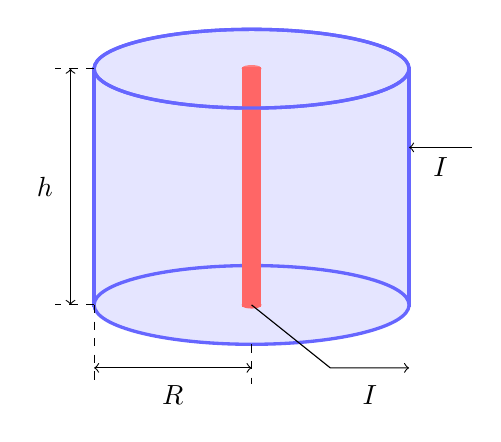
\begin{tikzpicture}
    %Vỏ ngoài
    \filldraw[color=blue!60, fill=blue!10, very thick] (-2,-1) rectangle (2,2);
    \filldraw[color=blue!60, fill=blue!10, very thick] (0,2) ellipse (2 and 0.5);
    \filldraw[color=blue!60, fill=blue!10, very thick] (0,-1) ellipse (2 and 0.5);
    %Vỏ trong
    \filldraw[color=red!50, fill=red!50, very thick] (0,2) ellipse (0.1 and 0.025);
    \filldraw[color=red!60, fill=red!60, very thick] (0,-1) ellipse (0.1 and 0.025);
    \filldraw[color=red!60, fill=red!60, very thick] (-0.1,-1) rectangle (0.1,2);
    %Tô thêm
    \draw[blue!60, very thick] (0,2) ellipse (2 and 0.5);
    %Thông số
    %h
    \draw[dashed] (-2,2)--(-2.5,2);
    \draw[dashed] (-2,-1)--(-2.5,-1);
    \draw[<->] (-2.3,2)--(-2.3,-1);
    \draw (-2.4,0.5) node[left]{$h$};
    %R
    \draw[dashed] (-2,-1)--(-2,-2);
    \draw[dashed] (0,-1.5)--(0,-2);
    \draw[<->] (-2,-1.8)--(0,-1.8);
    \draw (-1,-1.9) node[below]{$R$};
    %I
    \draw[->] (0,-1)--(1,-1.8)--(2,-1.8);
    \draw (1.5,-1.9) node[below]{$I$};
    \draw[->] (2.8,1)--(2,1);
    \draw (2.4,1) node[below]{$I$};
\end{tikzpicture}
\end{center}

\begin{enumerate}[label=\textbf{\alph*,}]\itemsep0em

\item Tìm biểu thức mật độ điện tích khối $\rho$ theo điện thế $V$ tại điểm có bán kính $r$ theo $h$, $I$, $e$, $m$, $r$.

\item Chứng minh rằng, điện thế $V(r)$ là nghiệm của phương trình vi phân:
$$\frac{1}{r} \frac{d}{dr} \left( r \frac{dV}{dr} \right) = \frac{\rho}{\varepsilon_0}.$$

\item Nghiệm của phương trình vi phân \textbf{b} sau khi thế điện trở suất tìm được ở phần \textbf{a} vào sẽ có dạng $V(r)=A r^\alpha$, trong đó $A$ và $\alpha$ là các hằng số không phụ thuộc vào $r$. Xác định các hệ số $A$ và $\alpha$ theo $I$, $e$, $m$, $\varepsilon_0$, $h$, $R$.

\item Theo định luật Child-Langmuir hay còn được gọi là "định luật số-mũ-ba-phần-hai" (three-halves-power law), khi bỏ qua vận tốc đầu của các electron khi bật ra, các diode chân không bất kể hình dạng nào cũng sẽ có đường đặc tuyến Volt-Ampere tuân theo biểu thức:
$$ I = K U^{3/2}.$$
Với $K$ là một hằng số. Chứng minh rằng trường hợp diode chân không hình trụ tuân theo định luật này. Xác định hệ số $K$ theo $e$, $m$, $\varepsilon_0$, $h$, $R$.
\end{enumerate}

\begin{flushright}
    (Biên soạn bởi Log)
\end{flushright}